To demonstrate the EP-LP transition, we can also consider an experiment on the implementation of a one-dimensional system \cite{schreiber_observation_2015} with degenerate Fermi gase of ${}^{40}$K via sympathetic cooling with ${}^{87}$Rb in a magnetic quadrupole and optical dipole trap followed by evaporative cooling. 

Now we consider the motion in a quasi-random optical lattice created by two gratings with an incommensurate step, but in general still described by the Hamiltonian close to \eqref{9:model}:
\begin{equation*}
         \hat{H} = - J \sum_{j,\sigma} \left(\hat{c}\D_{j,\sigma} \hat{c}_{j+1,\sigma} + \hc \right) + \Delta \sum_{j, \sigma} \cos(2 \pi \beta j + \varphi) \hat{n}_{j, \sigma} + U \sum_j \hat{n}_{j, \uparrow} \hat{n}_{j, \downarrow},
\end{equation*} 
with $\beta \in \mathbb{Q}$ to have quasi-random potential.  A general view of the phase diagram is presented in fig. \ref{fig:1Dmain}b.


Now odd nodes are chosen as $\Omega_1$ and we also study how quickly and to what extent the contrast $\mathcal{I}$ of the population of even and odd nodes will disappear (fig. \ref{fig:loc1D1}). It can be seen that for $t \approx 15 \tau$ the observed $\mathcal{I}$ also reaches a stationary value (fig. \ref{fig:loc1D1}a), where the dependence $\mathcal{I}(\Delta)$ (fig. \ref{fig:loc1D1}b) is plotted based on the results of averaging in the yellow region.

\begin{figure}[h]
    \centering
    \addletter{45}{a}
    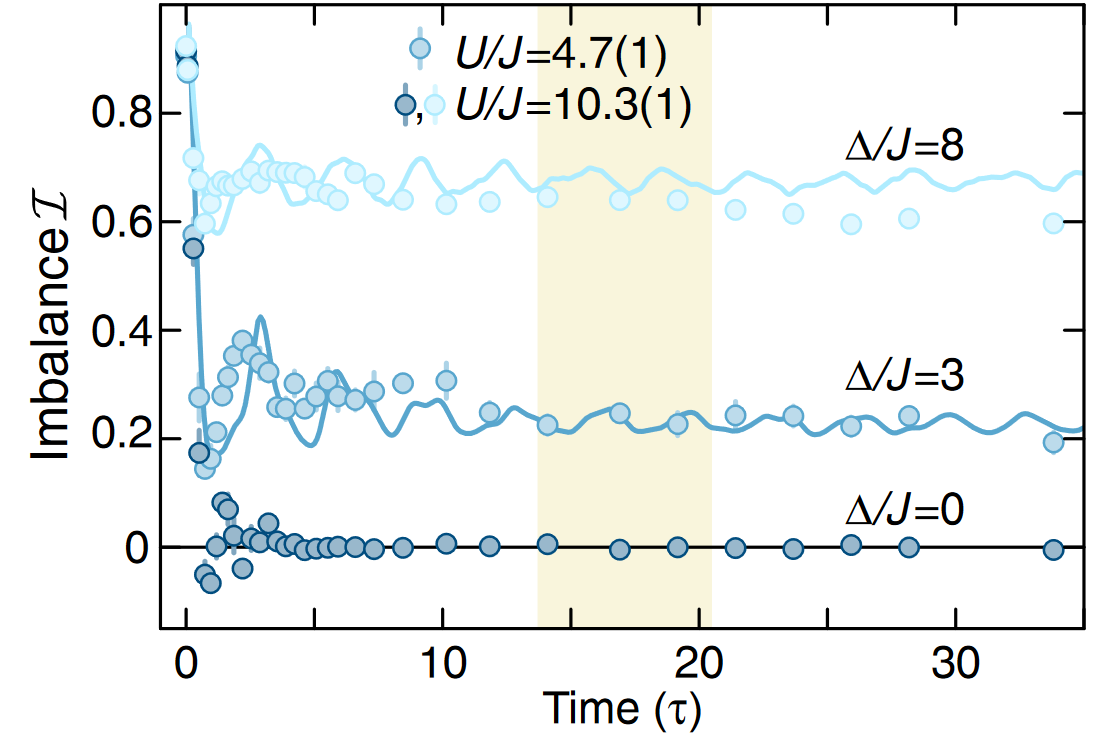
\includegraphics[align=c, width=0.35\textwidth]{imgs/MBL_exp_1.png}
    \hspace{10 mm} 
    \addletter{45}{b}
    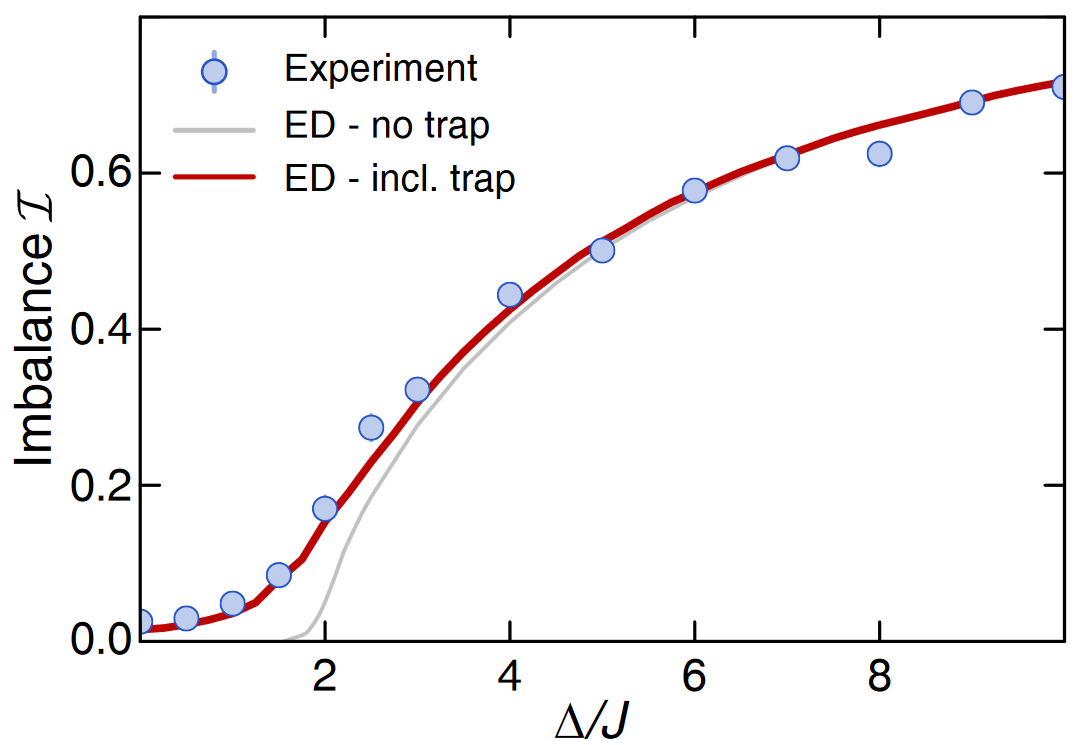
\includegraphics[align=c, width=0.35\textwidth]{imgs/MBL_exp_2.png}
    \caption{
    \cite{schreiber_observation_2015} 
    a) Time evolution of an initial charge-density wave
    . 
    b) Stationary values of the imbalance $\mathcal{I}$ as a function of disorder $\Delta$ for non-interacting atoms 
    .
    }
    \label{fig:loc1D1}
\end{figure} 

In the paper also measured the stationary value of $\mathcal{I}$ for different interactions $U$ and different noise $\Delta$ (fig. \ref{fig:1daddb}b), in full accordance with the results of DMRG simulation 
\cite{PhysRevLett.69.2863}. 
It can be seen that LP is preserved in a wide range of interactions. The effect of interactions on the localization gives rise to a characteristic W-shape. It is also worth noting that the interaction leads to a logarithmic increase in the entropy of entanglement of subsystems (DMRG results at fig. \ref{fig:1daddb}a)
, which we will return to in the corresponding section.



% \red{Основной вывод от этой картинки и этой статьи: есть локализация и термолизация. Взаимодействие влияет, но не столь принципиально.}}